% Created 2021-12-21 Tue 08:32
\documentclass[9pt, b5paper]{article}
\usepackage[UTF8]{ctex}
\usepackage{xltxtra}
\usepackage{bera}
\usepackage[T1]{fontenc}
\usepackage[scaled]{beraserif}
\usepackage[scaled]{berasans}
\usepackage[scaled]{beramono}
\usepackage{graphicx}
\usepackage{xcolor}
\usepackage{multirow}
\usepackage{multicol}
\usepackage{float}
\usepackage{textcomp}
\usepackage{geometry}
\geometry{left=1.2cm,right=1.2cm,top=1.5cm,bottom=1.2cm}
\usepackage{algorithm}
\usepackage{algorithmic}
\usepackage{latexsym}
\usepackage{natbib}
\usepackage{minted}
\newminted{common-lisp}{fontsize=ootnotesize}
\usepackage[xetex,colorlinks=true,CJKbookmarks=true,linkcolor=blue,urlcolor=blue,menucolor=blue]{hyperref}
\author{deepwaterooo}
\date{\today}
\title{Main Topics Specific}
\hypersetup{
  pdfkeywords={},
  pdfsubject={},
  pdfcreator={Emacs 27.1 (Org mode 8.2.7c)}}
\begin{document}

\maketitle
\tableofcontents


\section{Jetpack library}
\label{sec-1}
\begin{itemize}
\item \url{https://blog.csdn.net/Alexwll/article/details/83302173}
\item Android Jetpack组件的优势:
\begin{itemize}
\item 轻松管理应用程序的生命周期
\item 构建可观察的数据对象,以便在基础数据库更改时通知视图
\item 存储在应用程序轮换中未销毁的UI相关数据,在界面重建后恢复数据
\item 轻松的实现SQLite数据库
\item 系统自动调度后台任务的执行,优化使用性能
\item Android Jetpack组件推荐的使用项目架构
\end{itemize}
\end{itemize}

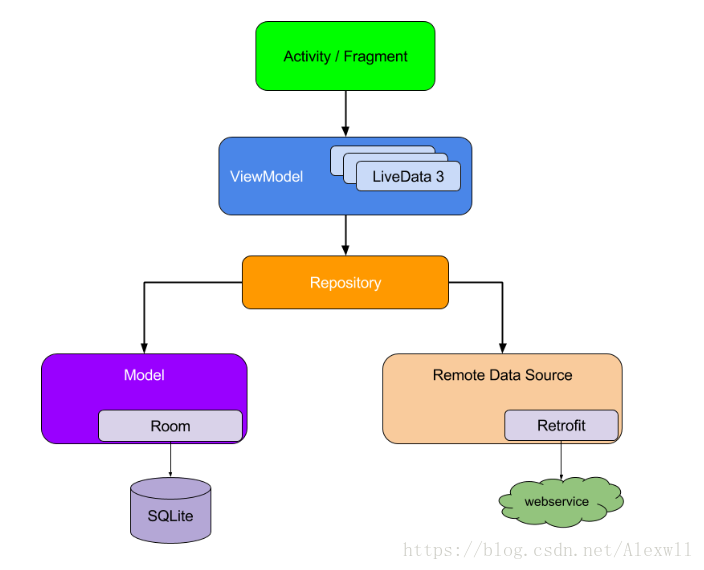
\includegraphics[width=.9\linewidth]{./pic/jetpack.png}

\begin{itemize}
\item 上面架构组件的功能如下:
\begin{itemize}
\item Activity和Fragment负责产品与用户的交互
\item ViewModel作为数据的存储和驱动
\item Resposity负责调度数据的获取
\item Room储存本地序列化的数据
\item Retrofit获取远程数据的数据
\end{itemize}
\end{itemize}


\section{JUnit Mockito Unit Testing}
\label{sec-2}
\begin{itemize}
\item 当您需要更快地运行测试而不需要与在真实设备上运行测试关联的保真度和置信度时,可以使用本地单元测试来评估应用的逻辑。对于这种方法,您通常使用 Robolectric 或模拟框架(如 Mockito)来实现依赖项。
\begin{itemize}
\item 如果您的测试对 Android 框架有依赖性(特别是与框架建立复杂互动的测试),最好使用 Robolectric 添加框架依赖项。
\item 如果您的测试对 Android 框架的依赖性极小,或者如果测试仅取决于您自己的对象,可以使用诸如 Mockito 之类的模拟框架添加模拟依赖项。
\end{itemize}
\end{itemize}
\begin{minted}[frame=lines,fontsize=\scriptsize,linenos=false]{groovy}
dependencies {
        // Required -- JUnit 4 framework
        testImplementation 'junit:junit:4.12'
        // Optional -- Robolectric environment
        testImplementation 'androidx.test:core:1.0.0'
        // Optional -- Mockito framework
        testImplementation 'org.mockito:mockito-core:1.10.19'
    }
\end{minted}
\begin{itemize}
\item 创建本地单元测试类
\begin{minted}[frame=lines,fontsize=\scriptsize,linenos=false]{java}
 import com.google.common.truth.Truth.assertThat;
    import org.junit.Test;
    public class EmailValidatorTest {
        @Test
        public void emailValidator_CorrectEmailSimple_ReturnsTrue() {
            assertThat(EmailValidator.isValidEmail("name@email.com")).isTrue();
        }
    }
\end{minted}
\item 添加框架依赖项 
\begin{itemize}
\item 如果您的测试与多个 Android 框架依赖项互动,或以复杂的方式与这些依赖项互动,请使用 AndroidX Test 提供的 Robolectric 工件。Robolectric 在本地 JVM 或真实设备上执行真实的 Android 框架代码和原生框架代码的虚假对象。
\item 以下示例展示了如何创建使用 Robolectric 的单元测试:
\end{itemize}
\end{itemize}
\begin{minted}[frame=lines,fontsize=\scriptsize,linenos=false]{groovy}
app/build.gradle
    android {
        // ...
        testOptions {
            unitTests.includeAndroidResources = true
        }
    }
\end{minted}
\begin{itemize}
\item 
\end{itemize}
\begin{minted}[frame=lines,fontsize=\scriptsize,linenos=false]{java}
    import android.content.Context;
    import androidx.test.core.app.ApplicationProvider;
    import org.junit.Test;
    import static com.google.common.truth.Truth.assertThat;
    public class UnitTestSampleJava {
        private static final String FAKE_STRING = "HELLO_WORLD";
        private Context context = ApplicationProvider.getApplicationContext();
        @Test
        public void readStringFromContext_LocalizedString() {
            // Given a Context object retrieved from Robolectric...
            ClassUnderTest myObjectUnderTest = new ClassUnderTest(context);
            // ...when the string is returned from the object under test...
            String result = myObjectUnderTest.getHelloWorldString();
            // ...then the result should be the expected one.
            assertThat(result).isEqualTo(FAKE_STRING);
        }
    }
\end{minted}
\begin{itemize}
\item 稍微复杂一点儿的
\end{itemize}
\begin{minted}[frame=lines,fontsize=\scriptsize,linenos=false]{java}
    import android.content.Context;
    import org.junit.Test;
    import org.junit.runner.RunWith;
    import org.mockito.Mock;
    import org.mockito.junit.MockitoJUnitRunner;
    import static com.google.common.truth.Truth.assertThat;
    import static org.mockito.Mockito.when;
    @RunWith(MockitoJUnitRunner.class)
    public class UnitTestSample {
        private static final String FAKE_STRING = "HELLO WORLD";
        @Mock
        Context mockContext;
        @Test
        public void readStringFromContext_LocalizedString() {
            // Given a mocked Context injected into the object under test...
            when(mockContext.getString(R.string.hello_world))
                    .thenReturn(FAKE_STRING);
            ClassUnderTest myObjectUnderTest = new ClassUnderTest(mockContext);
            // ...when the string is returned from the object under test...
            String result = myObjectUnderTest.getHelloWorldString();
            // ...then the result should be the expected one.
            assertThat(result, is(FAKE_STRING));
        }
    }
\end{minted}

\section{HttpURLConnection Retrofit2 Json Parsing}
\label{sec-3}
\subsection{常见的网络框架}
\label{sec-3-1}
\begin{itemize}
\item HttpURLConnection:  Android 2.2版本之前,HttpClient拥有较少的bug,因此使用它是***的选择。而在Android 2.3版本及以后,HttpURLConnection则是***的选择。它的API简单,体积较小,因而非常适用于Android项目。压缩和缓存机制可以有效地减少网络访问的流量,在提升速度和省电方面也起到了较大的作用。对于新的应用程序应该更加偏向于使用HttpURLConnection,因为在以后的工作当中我们也会将更多的时间放在优化HttpURLConnection上面。特点:比较轻便,灵活,易于扩展,在3.0后以及4.0中都进行了改善,如对HTTPS的支持,在4.0中,还增加了对缓存的支持。
\item HttpClient:高效稳定,但是维护成本高昂,故android 开发团队不愿意在维护该库而是转投更为轻便的
\item okHttp:okhttp 是一个 Java 的 HTTP+SPDY 客户端开发包,同时也支持 Android。需要Android 2.3以上。特点:OKHttp是Android版Http客户端。非常高效,支持SPDY、连接池、GZIP和 HTTP 缓存。默认情况下,OKHttp会自动处理常见的网络问题,像二次连接、SSL的握手问题。如果你的应用程序中集成了OKHttp,Retrofit默认会使用OKHttp处理其他网络层请求。从Android4.4开始HttpURLConnection的底层实现采用的是okHttp。
\item volley:早期使用HttpClient,后来使用HttpURLConnection,是谷歌2013年推出的网络请求框架,非常适合去进行数据量不大,但通信频繁的网络操作,而对于大数据量的网络操作,比如说下载文件等,Volley的表现就会非常糟糕。
\item xutils:缓存网络请求数据
\item Retrofit:和Volley框架的请求方式很相似,底层网络请求采用okhttp(效率高,android4.4底层采用okhttp),采用注解方式来指定请求方式和url地址,减少了代码量。
\end{itemize}
\subsection{Retrofit库的核心实现原理是什么?如果让你实现这个库的某些核心功能,你会考虑怎么去实现?}
\label{sec-3-2}
\begin{itemize}
\item Retrofit主要是在create方法中采用动态代理模式(通过访问代理对象的方式来间接访问目标对象)实现接口方法,这个过程构建了一个ServiceMethod对象,根据方法注解获取请求方式,参数类型和参数注解拼接请求的链接,当一切都准备好之后会把数据添加到Retrofit的RequestBuilder中。然后当我们主动发起网络请求的时候会调用okhttp发起网络请求,okhttp的配置包括请求方式,URL等在Retrofit 的RequestBuilder的build()方法中实现,并发起真正的网络请求。
\item 你从这个库中学到什么有价值的或者说可借鉴的设计思想?
\item 内部使用了优秀的架构设计和大量的设计模式,在我分析过Retrofit最新版的源码和大量优秀的Retrofit 源码分析文章后,我发现,要想真正理解Retrofit内部的核心源码流程和设计思想,首先,需要对它使用到的九大设计模式有一定的了解,下面我简单说一说:
\item 1、创建Retrofit实例: 使用 \uline{建造者模式} 通过内部Builder类建立了一个Retroift实例。 网络请求工厂使用了 \uline{工厂模式} 方法。
\item 2、创建网络请求接口的实例:
\begin{itemize}
\item 首先,使用 \uline{外观模式} 统一调用创建网络请求接口实例和网络请求参数配置的方法。 然后,使用 \uline{动态代理} 动态地去创建网络请求接口实例。
\item 接着,使用了 \uline{建造者模式} \& \uline{单例模式} 创建了serviceMethod对象。
\item 再者,使用了 \uline{策略模式} 对serviceMethod对象进行网络请求参数配置,即通过解析网络请求接口方 法的参数、返回值和注解类型,从Retrofit对象中获取对应的网络的url地址、网络请求执行器、网 络请求适配器和数据转换器。
\item 最后,使用了 \uline{装饰者模式} ExecuteCallBack为serviceMethod对象加入线程切换的操作,便于接受 数据后通过Handler从子线程切换到主线程从而对返回数据结果进行处理。
\end{itemize}
\item 3、发送网络请求: 在异步请求时,通过静态delegate代理对网络请求接口的方法中的每个参数使用对应的ParameterHanlder进行解析。
\item 4、解析数据
\item 5、切换线程: 使用了 \uline{适配器模式} 通过检测不同的Platform使用不同的回调执行器,然后使用回调执行器切换线程,这里同样是使用了装饰模式。
\item 6、处理结果
\end{itemize}


\section{SQLite Datebase}
\label{sec-4}


\section{RecyclerView}
\label{sec-5}
\subsection{RecyclerView与ListView}
\label{sec-5-1}
\begin{itemize}
\item RecyclerView与ListView的不同点,主要在于以下几个特性:
\begin{itemize}
\item Adapter中的ViewHolder模式,ListView没有严格的ViewHolder设计模式。但是在RecyclerView中,Adapter必须按照ViewHolder模式实现至少一个ViewHolder。
\item 定制Item视图,ListView只能实现垂直线性排列的列表视图。RecyclerView可以通过设置RecyclerView.LayoutManager来定制不同风格的视图,比如水平滚动列表或者不规则的瀑布流列表。
\item Item动画,在ListView中没有提供任何方法或者接口,以实现Item的增删动画。RecyclerView可以通过设置RecyclerView.ItemAnimator来为Item增加动画效果。
\item 设置数据源,在LisView中针对不同数据封装了各种类型的Adapter,比如用来处理数组的ArrayAdapter和用来展示Database结果的CursorAdapter。而RecyclerView中必须自定义实现RecyclerView.Adapter并为其提供数据集合。
\item 设置Item分割线,在ListView中可以通过设置android:divider属性来为两个Item间设置分割线。而RecyclerView必须使用RecyclerView.ItemDecoration,这种实现方式更灵活,样式也更加丰富。
\item 设置Item点击事件,在ListView中存在AdapterView.OnItemClickListener接口,用来绑定Item的点击事件。而RecyclerView并没有提供这样的接口,但是它提供了另外一个接口RcyclerView.OnItemTouchListener,用来响应Item的触摸事件。
\end{itemize}
\item RecyclerView的优点
\begin{itemize}
\item RecyclerView封装了viewholder的回收复用,也就是说RecyclerView标准化了ViewHolder,编写Adapter面向的是ViewHolder而不再是View了,复用的逻辑被封装了,写起来更加简单。
\item 直接省去了listview中convertView.setTag(holder)和convertView.getTag()这些繁琐的步骤。
\item 提供了一种插拔式的体验,高度的解耦,异常的灵活,针对一个Item的显示RecyclerView专门抽取出了相应的类,来控制Item的显示,使其的扩展性非常强。
\item 设置布局管理器以控制Item的布局方式,横向、竖向以及瀑布流方式
\begin{itemize}
\item 例如:你想控制横向或者纵向滑动列表效果可以通过LinearLayoutManager这个类来进行控制(与GridView效果对应的是GridLayoutManager,与瀑布流对应的还StaggeredGridLayoutManager等)。也就是说RecyclerView不再拘泥于ListView的线性展示方式,它也可以实现GridView的效果等多种效果。
\end{itemize}
\item 可设置Item的间隔样式(可绘制)
\item 通过继承RecyclerView的ItemDecoration这个类,然后针对自己的业务需求去书写代码。
\item 可以控制Item增删的动画,可以通过ItemAnimator这个类进行控制,当然针对增删的动画,RecyclerView有其自己默认的实现。
\end{itemize}
\end{itemize}

\subsection{如果你想使用RecyclerView,需要做以下操作:}
\label{sec-5-2}
\begin{itemize}
\item RecyclerView.Adapter - 处理数据集合并负责绑定视图
\item ViewHolder - 持有所有的用于绑定数据或者需要操作的View
\item LayoutManager - 负责摆放视图等相关操作
\item ItemDecoration - 负责绘制Item附近的分割线
\item ItemAnimator - 为Item的一般操作添加动画效果,如,增删条目等
\end{itemize}

\subsection{主要部件}
\label{sec-5-3}
\subsubsection{Adapter}
\label{sec-5-3-1}
\begin{itemize}
\item 在RecylerView中,Adapter扮演着两个角色:一是根据不同viewType创建与之相应的的itemView,二是访问数据集合并将数据绑定到正确的View上。这就需要我们实现以下两个函数:
\end{itemize}
\begin{minted}[frame=lines,fontsize=\scriptsize,linenos=false]{java}
public ViewHolder onCreateViewHolder(ViewGroup parent, int viewType); // 创建Item视图,并返回相应的ViewHolder
public void onBindViewHolder(ViewHolder holder, int position);        // 绑定数据到正确的Item视图上
\end{minted}
\begin{itemize}
\item 另外我们还需要重写另一个方法,像ListView-Adapter那样,同样地告诉RecyclerView-Adapter列表Items的总数:
\end{itemize}
\begin{minted}[frame=lines,fontsize=\scriptsize,linenos=false]{java}
public int getItemCount(); // 返回该Adapter所持有的Itme数量
\end{minted}
\subsubsection{ViewHolder}
\label{sec-5-3-2}
\begin{itemize}
\item ViewHolder描述RecylerView中某个位置的itemView和元数据信息,属于Adapter的一部分,其实现类通常用于保存findViewById的结果。 主要元素组成有:
\end{itemize}
\begin{minted}[frame=lines,fontsize=\scriptsize,linenos=false]{java}
public static abstract class ViewHolder {
    View itemView;// itemView
    int mPosition;// 位置
    int mOldPosition;// 上一次的位置
    long mItemId;// itemId
    int mItemViewType;// itemViewType
    int mPreLayoutPosition;
    int mFlags;// ViewHolder的状态标志
    int mIsRecyclableCount;
    Recycler mScrapContainer;// 若非空,表明当前ViewHolder对应的itemView可以复用
}
\end{minted}
\begin{itemize}
\item 关于ViewHolder,这里主要介绍mFlags:
\begin{itemize}
\item FLAG\underBOUND——ViewHolder已经绑定到某个位置,mPosition、mItemId、mItemViewType都有效
\item FLAG\underUPDATE——ViewHolder绑定的View对应的数据过时需要重新绑定,mPosition、mItemId还是一致的
\item FLAG\underINVALID——ViewHolder绑定的View对应的数据无效,需要完全重新绑定不同的数据
\item FLAG\underREMOVED——ViewHolder对应的数据已经从数据集移除
\item FLAG\underNOT\underRECYCLABLE——ViewHolder不能复用
\item FLAG\underRETURNED\underFROM\underSCRAP——这个状态的ViewHolder会加到scrap list被复用。
\item FLAG\underCHANGED——ViewHolder内容发生变化,通常用于表明有ItemAnimator动画
\item FLAG\underIGNORE——ViewHolder完全由LayoutManager管理,不能复用
\item FLAG\underTMP\underDETACHED——ViewHolder从父RecyclerView临时分离的标志,便于后续移除或添加回来
\item FLAG\underADAPTER\underPOSITION\underUNKNOWN——ViewHolder不知道对应的Adapter的位置,直到绑定到一个新位置
\item FLAG\underADAPTER\underFULLUPDATE——方法addChangePayload(null)调用时设置
\end{itemize}
\end{itemize}
\begin{enumerate}
\item RecyclerView为什么强制我们实现ViewHolder模式?
\label{sec-5-3-2-1}
\begin{itemize}
\item ListView使用ViewHolder的好处就在于可以避免每次getView都进行findViewById()操作,因为findViewById()利用的是DFS算法(深度优化搜索),是非常耗性能的.
\item 而对于RecyclerView来说,强制实现ViewHolder的其中一个原因就是避免多次进行findViewById()的处理;另一个原因就是因为ItemView和ViewHolder的关系是一对一,也就是说一个ViewHolder对应一个ItemView。这个ViewHolder当中持有对应的ItemView的所有信息,比如说:position;view;width等等,拿到了ViewHolder基本就拿到了ItemView的所有信息,而ViewHolder使用起来相比itemView更加方便。
\item RecyclerView缓存机制缓存的就是ViewHolder(ListView缓存的是ItemView),这也是为什么RecyclerView为什么强制我们实现ViewHolder的原因。
\end{itemize}
\end{enumerate}

\subsubsection{LayoutManager}
\label{sec-5-3-3}
\begin{itemize}
\item LayoutManager主要作用是,测量和摆放RecyclerView中itemView,以及当itemView对用户不可见时循环复用处理。
\item 布局管理器:RecyclerView.LayoutManager
\item 上述代码中mLayoutManager 对象是布局管理器,RecyclerView提供了三种布局管理器:
\begin{itemize}
\item LinerLayoutManager(线性):以垂直或者水平列表方式展示Item
\item GridLayoutManager (网格):以网格方式展示Item
\item StaggeredGridLayoutManager(瀑布流): 以瀑布流方式展示Item
\end{itemize}
\end{itemize}
\begin{minted}[frame=lines,fontsize=\scriptsize,linenos=false]{java}
// LinearLayoutManager是用来做列表布局,也就是单列的列表
LinearLayoutManager linearLayoutManager = new LinearLayoutManager(this);
// 设置为垂直布局,默认是垂直的(垂直:LinearLayoutManager.VERTICAL,水平:LinearLayoutManager.HORIZONTAL)
linearLayoutManager.setOrientation(LinearLayoutManager.HORIZONTAL);
// 设置布局管理器
rvView.setLayoutManager(linearLayoutManager);

// 设置网格布局
GridLayoutManager gridLayoutManager = new GridLayoutManager(this, 4); //  第二个参数,行数或是列数,瀑布流布局类似
// 设置布局管理器
rvView.setLayoutManager(gridLayoutManager);

// 设置竖直瀑布流布局
StaggeredGridLayoutManager staggeredGridLayoutManager = new StaggeredGridLayoutManager(4, StaggeredGridLayoutManager.VERTICAL);
// 设置布局管理器
rvView.setLayoutManager(staggeredGridLayoutManager);
\end{minted}

\subsubsection{ItemDecoration: 间隔样式:RecyclerView.ItemDecoration}
\label{sec-5-3-4}
\begin{itemize}
\item 当我们想在某些item上加一些特殊的UI时,往往都是在itemView中先布局好,然后通过设置可见性来决定哪些位置显示不显示。RecyclerView将itemView和装饰UI分隔开来,装饰UI即ItemDecoration,主要用于绘制item间的分割线、高亮或者margin等。其源码如下:
\end{itemize}
\begin{minted}[frame=lines,fontsize=\scriptsize,linenos=false]{java}
public static abstract class ItemDecoration {
    // itemView绘制之前绘制,通常这部分UI会被itemView盖住
    public void onDraw(Canvas c, RecyclerView parent, State state) {
        onDraw(c, parent);
    }
    // itemView绘制之后绘制,这部分UI盖在itemView上面
    public void onDrawOver(Canvas c, RecyclerView parent, State state) {
        onDrawOver(c, parent);
    }
    // 设置itemView上下左右的间距
    public void getItemOffsets(Rect outRect, View view, RecyclerView parent, State state) {
        getItemOffsets(outRect, ((LayoutParams) view.getLayoutParams()).getViewLayoutPosition(), parent);
    }
}
\end{minted}
\begin{itemize}
\item 用于绘制itemView之间的一些特殊UI,比如在itemView之前设置空白区域、画线等。
\item RecyclerView 将itemView和装饰UI分隔开来,装饰UI即 ItemDecoration ,主要用于绘制item间的分割线、高亮或者margin等
\item 通过recyclerView.addItemDecoration(new DividerDecoration(this))对item添加装饰;对RecyclerView设置多个ItemDecoration,列表展示的时候会遍历所有的ItemDecoration并调用里面的绘制方法,对Item进行装饰。
\end{itemize}
\begin{minted}[frame=lines,fontsize=\scriptsize,linenos=false]{java}
public void onDraw(Canvas c, RecyclerView parent)     // 装饰的绘制在Item条目绘制之前调用,所以这有可能被Item的内容所遮挡
public void onDrawOver(Canvas c, RecyclerView parent) // 装饰的绘制在Item条目绘制之后调用,因此装饰将浮于Item之上
// 与padding或margin类似,LayoutManager在测量阶段会调用该方法,计算出每一个Item的正确尺寸并设置偏移量
public void getItemOffsets(Rect outRect, int itemPosition, RecyclerView parent)
\end{minted}
自定义间隔样式需要继承RecyclerView.ItemDecoration类,该类是个抽象类,主要有三个方法
\begin{minted}[frame=lines,fontsize=\scriptsize,linenos=false]{java}
onDraw(Canvas c, RecyclerView parent, State state)     // 在Item绘制之前被调用,该方法主要用于绘制间隔样式
onDrawOver(Canvas c, RecyclerView parent, State state) // 在Item绘制之前被调用,该方法主要用于绘制间隔样式
// 设置item的偏移量,偏移的部分用于填充间隔样式,在RecyclerView的onMesure()中会调用该方法
getItemOffsets(Rect outRect, View view, RecyclerView parent, State state)
\end{minted}
\begin{itemize}
\item onDraw()和onDrawOver()这两个方法都是用于绘制间隔样式,我们只需要复写其中一个方法即可。直接来看一下自定义的间隔样式的实现,参考官方实例, 然后在代码中设置RecyclerView的间隔样式
\end{itemize}

\subsubsection{ItemAnimator}
\label{sec-5-3-5}
\begin{itemize}
\item 过去AdapterView的item项操作往往是没有动画的。现在RecyclerView的ItemAnimator使得item的动画实现变得简单而样式丰富,我们可以自定义item项不同操作(如添加,删除)的动画效果。
\item RecyclerView做了一个notifyItemChanged()的操作,功能都顺利实现,问题当前Item闪烁,QA甚至为此提了Bug。闪烁主要由于RecyclerView使用的默认的动画导致的,所以解决的方法就是修改默认的动画。
\end{itemize}
\begin{enumerate}
\item 问题解决
\label{sec-5-3-5-1}
\begin{enumerate}
\item 更新部分item
\label{sec-5-3-5-1-1}
\begin{itemize}
\item (1)个别更新
\end{itemize}
\begin{minted}[frame=lines,fontsize=\scriptsize,linenos=false]{java}
imgAdapter.notifyItemChanged(i); // 只更新修改的item
\end{minted}
\begin{itemize}
\item (2)删除某个
\end{itemize}
\begin{minted}[frame=lines,fontsize=\scriptsize,linenos=false]{java}
selectedImgs.remove(position);
notifyItemRemoved(position);
notifyItemRangeChanged(0, selectedImgs.size());
\end{minted}
\item 屏蔽动画方法
\label{sec-5-3-5-1-2}
\begin{itemize}
\item DefaultItemAnimator继承自SimpleItemAnimator,里面有个方法是:
\end{itemize}
\begin{minted}[frame=lines,fontsize=\scriptsize,linenos=false]{java}
    /**
     * Sets whether this ItemAnimator supports animations of item change events.
     * If you set this property to false, actions on the data set which change the
     * contents of items will not be animated. What those animations do is left
     * up to the discretion of the ItemAnimator subclass, in its
     * {@link #animateChange(ViewHolder, ViewHolder, int, int, int, int)} implementation.
     * The value of this property is true by default.
     *
     */
    public void setSupportsChangeAnimations(boolean supportsChangeAnimations) {
        mSupportsChangeAnimations = supportsChangeAnimations;
    }
\end{minted}
\begin{itemize}
\item 只要设置为false,就可以不显示动画了,也就解决了闪烁问题。 关键代码:
\end{itemize}
\begin{minted}[frame=lines,fontsize=\scriptsize,linenos=false]{java}
((SimpleItemAnimator)recyclerView.getItemAnimator()).setSupportsChangeAnimations(false);
\end{minted}
\item 设置动画执行时间为0来解决闪烁问题: (这个效率会不会比较低?)
\label{sec-5-3-5-1-3}
\begin{minted}[frame=lines,fontsize=\scriptsize,linenos=false]{java}
recyclerView.getItemAnimator().setChangeDuration(0);// 通过设置动画执行时间为0来解决闪烁问题
\end{minted}
\item 修改默认的动画方法
\label{sec-5-3-5-1-4}
\begin{minted}[frame=lines,fontsize=\scriptsize,linenos=false]{java}
// 1.定义动画类
public class NoAlphaItemAnimator extends SimpleItemAnimator {
}
// 2.将DefaultItemAnimator类里的代码全部copy到自己写的动画类中,然后做一些修改。
// 3.首先找到private void animateChangeImpl(final ChangeInfo changeInfo) {}方法。
// 4.找到方法里这两句代码:
//    4.1 去掉alpha(0)
oldViewAnim.alpha(0).setListener(new VpaListenerAdapter() {...}).start();
oldViewAnim.setListener(new VpaListenerAdapter() {...}).start();
//    4.2 去掉alpha(1)
newViewAnimation.translationX(0).translationY(0).setDuration(getChangeDuration()).
                    alpha(1).setListener(new VpaListenerAdapter() {...}).start();
newViewAnimation.translationX(0).translationY(0).setDuration(getChangeDuration()).
                    setListener(new VpaListenerAdapter() {...}).start();
// 5.最后使用修改后的动画
recyclerView.setItemAnimator(new NoAlphaItemAnimator());
\end{minted}
\end{enumerate}
\end{enumerate}

\subsubsection{刷新方法}
\label{sec-5-3-6}
除了adapter.notifyDataSetChanged()这个方法之外,新的Adapter还提供了其他的方法,如下:
\begin{minted}[frame=lines,fontsize=\scriptsize,linenos=false]{java}
// 刷新所有
public final void notifyDataSetChanged();
// position数据发生了改变,那调用这个方法,就会回调对应position的onBindViewHolder()方法了
public final void notifyItemChanged(int position);
// 刷新从positionStart开始itemCount数量的item了(这里的刷新指回调onBindViewHolder()方法)
public final void notifyItemRangeChanged(int positionStart, int itemCount);

// 在第position位置被插入了一条数据的时候可以使用这个方法刷新,注意这个方法调用后会有插入的动画,这个动画可以使用默认的,也可以自己定义
public final void notifyItemInserted(int position);
// 从fromPosition移动到toPosition为止的时候可以使用这个方法刷新
public final void notifyItemMoved(int fromPosition, int toPosition);
// 批量添加
public final void notifyItemRangeInserted(int positionStart, int itemCount);
// 第position个被删除的时候刷新,同样会有动画
public final void notifyItemRemoved(int position);
// 批量删除
public final void notifyItemRangeRemoved(int positionStart, int itemCount);
\end{minted}

\subsubsection{Recycler}
\label{sec-5-3-7}
\begin{itemize}
\item Recycler用于管理已经废弃或与RecyclerView分离的(scrapped or detached)item view,便于重用。Scrapped view指依附于RecyclerView,但被标记为可移除或可复用的view。
\item LayoutManager获取Adapter某一项的View时会使用Recycler。当复用的View有效(clean)时,View能直接被复用,反之若View失效(dirty)时,需要重新绑定View。对于有效的View,如果不主动调用request layout,则不需要重新测量大小就能复用。在分析Recycler的复用原理之前,我们先了解下如下两个类:
\end{itemize}
\subsubsection{RecycledViewPool}
\label{sec-5-3-8}
\begin{itemize}
\item RecyclerViewPool用于多个RecyclerView之间共享View。只需要创建一个RecyclerViewPool实例,然后调用RecyclerView的setRecycledViewPool(RecycledViewPool)方法即可。RecyclerView默认会创建一个RecyclerViewPool实例。
\item 首先我们看一下ReyclerPool的结构。
\end{itemize}
\begin{minted}[frame=lines,fontsize=\scriptsize,linenos=false]{java}
public static class RecycledViewPool {
    private static final int DEFAULT_MAX_SCRAP = 5;
    static class ScrapData {
        ArrayList<ViewHolder> mScrapHeap = new ArrayList<>();
        int mMaxScrap = DEFAULT_MAX_SCRAP;
        long mCreateRunningAverageNs = 0;
        long mBindRunningAverageNs = 0;
    }
    SparseArray<ScrapData> mScrap = new SparseArray<>();
}
\end{minted}
\begin{itemize}
\item 可以看到RecyclerPool内部其实是一个SparseArray,可想而知,key就是我们的ViewType,而Value是ArrayList<ViewHolder>。
\item 我们来看一下RecyclerPool的put方法。
\end{itemize}
\begin{minted}[frame=lines,fontsize=\scriptsize,linenos=false]{java}
public void putRecycledView(ViewHolder scrap) {
    final int viewType = scrap.getItemViewType();
    final ArrayList<ViewHolder> scrapHeap = getScrapDataForType(viewType).mScrapHeap;
    if (mScrap.get(viewType).mMaxScrap <= scrapHeap.size()) 
        return;
    if (DEBUG && scrapHeap.contains(scrap)) 
        throw new IllegalArgumentException("this scrap item already exists");
    //重置ViewHolder
    scrap.resetInternal();
    scrapHeap.add(scrap);
}
\end{minted}
\begin{itemize}
\item 其中resetInternal方法值得我们注意。
\end{itemize}
\begin{minted}[frame=lines,fontsize=\scriptsize,linenos=false]{java}
void resetInternal() {
    mFlags = 0;
    mPosition = NO_POSITION;
    mOldPosition = NO_POSITION;
    mItemId = NO_ID;
    mPreLayoutPosition = NO_POSITION;
    mIsRecyclableCount = 0;
    mShadowedHolder = null;
    mShadowingHolder = null;
    clearPayload();
    mWasImportantForAccessibilityBeforeHidden = ViewCompat.IMPORTANT_FOR_ACCESSIBILITY_AUTO;
    mPendingAccessibilityState = PENDING_ACCESSIBILITY_STATE_NOT_SET;
    clearNestedRecyclerViewIfNotNested(this);
}
\end{minted}
\begin{itemize}
\item 可以看到所有被put进入RecyclerPool中的ViewHolder都会被重置,这也就意味着RecyclerPool中的ViewHolder再被复用的时候是需要重新Bind的。这一点就可以区分和CacheViews中缓存的区别。
\end{itemize}

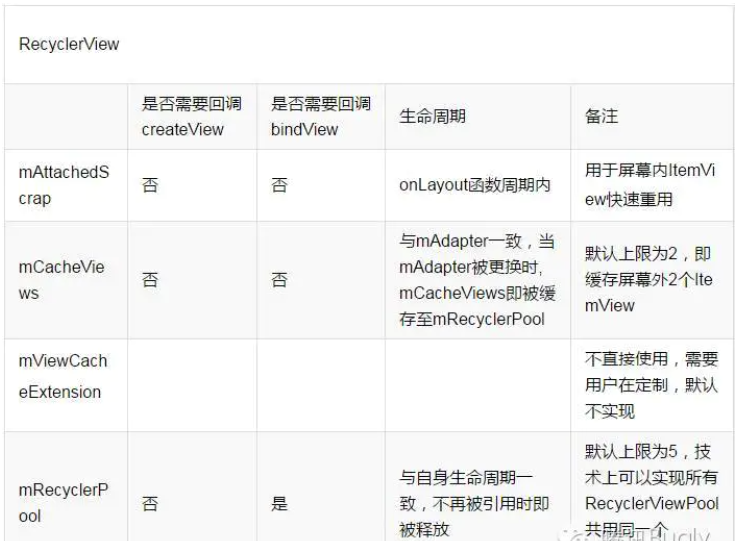
\includegraphics[width=.9\linewidth]{./pic/cache.png}

\begin{minted}[frame=lines,fontsize=\scriptsize,linenos=false]{java}
public static class RecycledViewPool { 
    private SparseArray<ArrayList<ViewHolder>> mScrap = new SparseArray<ArrayList<ViewHolder>>(); //  SparseArray 应用的实例
    private SparseIntArray mMaxScrap = new SparseIntArray();
    private int mAttachCount = 0;
    private static final int DEFAULT_MAX_SCRAP = 5;

    public void clear() {
        mScrap.clear();
    }
    public void setMaxRecycledViews(int viewType, int max) {
        mMaxScrap.put(viewType, max);
        final ArrayList<ViewHolder> scrapHeap = mScrap.get(viewType);
        if (scrapHeap != null) 
            while (scrapHeap.size() > max) 
                scrapHeap.remove(scrapHeap.size() - 1);
    }
    public ViewHolder getRecycledView(int viewType) {
        final ArrayList<ViewHolder> scrapHeap = mScrap.get(viewType);
        if (scrapHeap != null && !scrapHeap.isEmpty()) {
            final int index = scrapHeap.size() - 1;
            final ViewHolder scrap = scrapHeap.get(index);
            scrapHeap.remove(index);
            return scrap;
        }
        return null;
    }
    int size() {
        int count = 0;
        for (int i = 0; i < mScrap.size(); i ++) {
            ArrayList<ViewHolder> viewHolders = mScrap.valueAt(i);
            if (viewHolders != null) 
                count += viewHolders.size();
        }
        return count;
    }
    public void putRecycledView(ViewHolder scrap) {
        final int viewType = scrap.getItemViewType();
        final ArrayList scrapHeap = getScrapHeapForType(viewType);
        if (mMaxScrap.get(viewType) <= scrapHeap.size()) 
            return;
        if (DEBUG && scrapHeap.contains(scrap)) 
            throw new IllegalArgumentException("this scrap item already exists");
        scrap.resetInternal();
        scrapHeap.add(scrap);
    }
    void attach(Adapter adapter) {
        mAttachCount++;
    }
    void detach() {
        mAttachCount--;
    }
    /**
     * Detaches the old adapter and attaches the new one.
     * <p>
     * RecycledViewPool will clear its cache if it has only one adapter attached and the new
     * adapter uses a different ViewHolder than the oldAdapter.
     *
     * @param oldAdapter The previous adapter instance. Will be detached.
     * @param newAdapter The new adapter instance. Will be attached.
     * @param compatibleWithPrevious True if both oldAdapter and newAdapter are using the same
     *                               ViewHolder and view types.
     */
    void onAdapterChanged(Adapter oldAdapter, Adapter newAdapter, boolean compatibleWithPrevious) {
        if (oldAdapter != null) 
            detach();
        if (!compatibleWithPrevious && mAttachCount == 0) 
            clear();
        if (newAdapter != null) 
            attach(newAdapter);
    }
    private ArrayList<ViewHolder> getScrapHeapForType(int viewType) {
        ArrayList<ViewHolder> scrap = mScrap.get(viewType);
        if (scrap == null) {
            scrap = new ArrayList<ViewHolder>();
            mScrap.put(viewType, scrap);
            if (mMaxScrap.indexOfKey(viewType) < 0) 
                mMaxScrap.put(viewType, DEFAULT_MAX_SCRAP);
        }
        return scrap;
    }
}
\end{minted}
\begin{itemize}
\item 通过源码我们可以看出mScrap是一个<viewType, List>的映射,mMaxScrap是一个<viewType, maxNum>的映射,这两个成员变量代表可复用View池的基本信息。调用setMaxRecycledViews(int viewType, int max)时,当用于复用的mScrap中viewType对应的ViewHolder个数超过maxNum时,会从列表末尾开始丢弃超过的部分。调用getRecycledView(int viewType)方法时从mScrap中移除并返回viewType对应的List的末尾项。
\end{itemize}

\subsubsection{ViewCacheExtension}
\label{sec-5-3-9}
\begin{itemize}
\item ViewCacheExtension是一个由开发者控制的可以作为View缓存的帮助类。调用Recycler.getViewForPosition(int)方法获取View时,Recycler先检查attached scrap和一级缓存,如果没有则检查ViewCacheExtension.getViewForPositionAndType(Recycler, int, int),如果没有则检查RecyclerViewPool。注意:Recycler不会在这个类中做缓存View的操作,是否缓存View完全由开发者控制。
\end{itemize}
\begin{minted}[frame=lines,fontsize=\scriptsize,linenos=false]{java}
public abstract static class ViewCacheExtension {
    abstract public View getViewForPositionAndType(Recycler recycler, int position, int type);
}
\end{minted}
\begin{itemize}
\item 现在大家熟悉了RecyclerViewPool和ViewCacheExtension的作用后,下面开始介绍Recycler。
\item 如下是Recycler的几个关键成员变量和方法:
\end{itemize}
\begin{minted}[frame=lines,fontsize=\scriptsize,linenos=false]{java}
private ArrayList<ViewHolder> mAttachedScrap;
private ArrayList<ViewHolder> mChangedScrap; // 与RecyclerView分离的ViewHolder列表。
private ArrayList<ViewHolder> mCachedViews;  // ViewHolder缓存列表。
private ViewCacheExtension mViewCacheExtension; // 开发者控制的ViewHolder缓存
private RecycledViewPool mRecyclerPool; // 提供复用ViewHolder池。
public void bindViewToPosition(View view, int position); // 将某个View绑定到Adapter的某个位置。
public View getViewForPosition(int position);
\end{minted}
\begin{itemize}
\item 获取某个位置需要展示的View,先检查是否有可复用的View,没有则创建新View并返回。具体过程为:
\begin{itemize}
\item 检查mChangedScrap,若匹配到则返回相应holder
\item 检查mAttachedScrap,若匹配到、且holder有效则返回相应holder
\item 检查mViewCacheExtension,若匹配到则返回相应holder
\item 检查mRecyclerPool,若匹配到则返回相应holder
\item 否则执行Adapter.createViewHolder(),新建holder实例
\item 返回holder.itemView
\end{itemize}
\item 注:以上每步匹配过程都可以匹配position或itemId(如果有stableId)。
\end{itemize}

\subsection{RecyclerView的缓存机制}
\label{sec-5-4}
\begin{itemize}
\item \url{https://www.jianshu.com/p/3e9aa4bdaefd} 希望能更深入地理解一下缓存机制
\item ListView的缓存机制:
\begin{itemize}
\item listView 是继承于 AbsListView ,RecycleBin 是 AbsListView 的内部类,其作用是通过两级缓存来缓存 view。
\item 一级缓存:mActiveViews
\begin{itemize}
\item 第一级缓存,这些 View 是布局过程开始时屏幕上的 view,layout 开始时这个数组被填充,layout 结束,mActiveViews 中的 View 移动到 mScrapView,意义在于快速重用屏幕上可见的列表项 ItemView,而不需要重新 createView 和 bindView。Active View:是缓存在屏幕内的ItemView,当列表数据发生变化时,屏幕内的数据可以直接拿来复用,无须进行数据绑定。
\end{itemize}
\item 二级缓存:mScrapView
\begin{itemize}
\item 第二级缓存,mScrapView 是多个 List 组成的数据,数组的长度为 viewTypeCount,每个 List 缓存不同类型 Item 布局的 View,其意义在于缓存离开屏幕的 ItemView,目的是让即将进入屏幕的 itemView 重用,当 mAdapter 被更换时,mScrapViews 则被清空。Scrap view:缓存屏幕外的ItemView,这里所有的缓存的数据都是"脏的",也就是数据需要重新绑定,也就是说屏幕外的所有数据在进入屏幕的时候都要走一遍getView()方法。当Active View和Scrap View中都没有缓存的时候就会直接create view。
\item 再来一张图,看看ListView的缓存流程
\end{itemize}
\end{itemize}
\end{itemize}

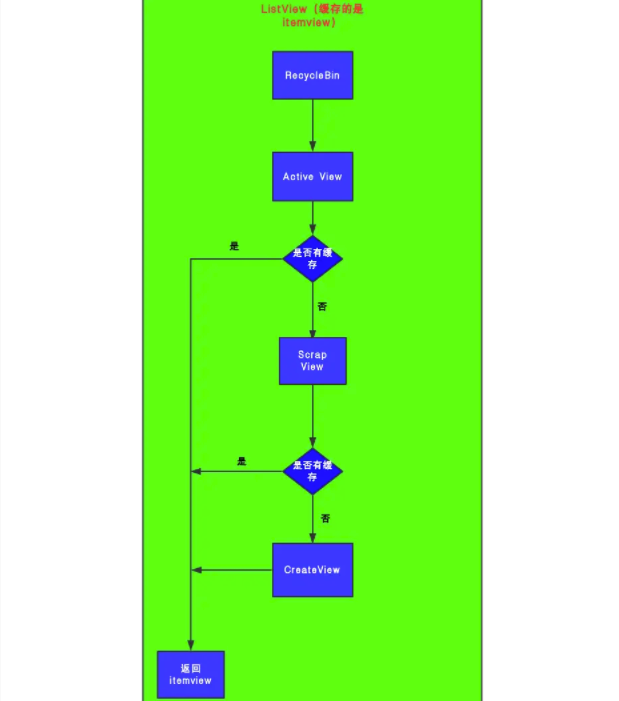
\includegraphics[width=.9\linewidth]{./pic/listviewcache.png}

\begin{itemize}
\item RecyclerView 也有一个类专门来管理缓存,不过与 ListView 不同的是,RecylerView 缓存的是 ViewHolder,而且实现的是四级缓存。
\begin{itemize}
\item 一级:Scrap
\begin{itemize}
\item 对应ListView 的一级缓存,快速重用屏幕上可见的 ViewHolder。
\item 简而言之,屏幕内显示的。
\end{itemize}
\item 二级:Cached
\begin{itemize}
\item 对应ListView的二级缓存,如果仍依赖于 RecyclerView(比如已经滑出可视范围,但还没有被移除掉),但已经被标记移除的 ItemView 集合被添加到 mAttachedScrap 中。然后如果 mAttachedScrap 中不再依赖时会被加入到 mCachedViews 中,默认缓存 2 个 ItemView,RecycleView 从这里获取的缓存时,如果数据源不变的情况下,无需重新 bindView。
\item 简而言之,linearlayoutmanager来说cached缓存默认大小为2,起到的作用就是rv滑动时刚被移出屏幕的viewholer的收容所。
\end{itemize}
\item 三级:CacheExtension
\begin{itemize}
\item 第三级缓存,其实是一个抽象静态类,用于充当附加的缓存池,当 RecyclerView 从 mCacheViews 找不到需要的 View 时,将会从 ViewCacheExtension 中寻找。不过这个缓存是由开发者维护的,如果没有设置它,则不会启用。通常我们也不会设置它,除非有特殊需求,比如要在调用系统的缓存池之前,返回一个特定的视图,才会用到它。
\item 简而言之,这是一个自定义的缓存,没错rv是可以自定义缓存行为的。
\item 目前来说这还只是个空实现而已,从这点来看其实rv所说的四级缓存本质上还只是三级缓存。
\end{itemize}
\item 四级:RecycledViewPool(最强大)
\begin{itemize}
\item 它是一个缓存池,实现上,是通过一个默认为 5 大小的 ArrayList 实现的。这一点,同 ListView 的 RecyclerBin 这个类一样。每一个 ArrayList 又都是放在一个 Map 里面的,SparseArray 用两个数组用来替代 Map。
\item 把所有的 ArrayList 放在一个 Map 里面,这也是 RecyclerView 最大的亮点,这样根据 itemType 来取不同的缓存 Holder,每一个 Holder 都有对应的缓存,而只需要为这些不同 RecyclerView 设置同一个 Pool 就可以了。
\item 简而言之, pool一般会和cached配合使用,这么来说,cached存不下的会被保存到pool中毕竟cached默认容量大小只有2,但是pool容量 也是有限的当保存满之后再有viewholder到来的话就只能会无情抛弃掉,它也有一个默认的容量大小
\end{itemize}
\item Scrap对应ListView 的Active View,就是屏幕内的缓存数据,就是相当于换了个名字,可以直接拿来复用。
\item Cache 刚刚移出屏幕的缓存数据,默认大小是2个,当其容量被充满同时又有新的数据添加的时候,会根据FIFO原则,把优先进入的缓存数据移出并放到下一级缓存中,然后再把新的数据添加进来。Cache里面的数据是干净的,也就是携带了原来的ViewHolder的所有数据信息,数据可以直接来拿来复用。需要注意的是,cache是根据position来寻找数据的,这个postion是根据第一个或者最后一个可见的item的position以及用户操作行为(上拉还是下拉)。
\begin{itemize}
\item 举个栗子:当前屏幕内第一个可见的item的position是1,用户进行了一个下拉操作,那么当前预测的position就相当于(1-1=0),也就是position=0的那个item要被拉回到屏幕,此时RecyclerView就从Cache里面找position=0的数据,如果找到了就直接拿来复用。
\end{itemize}
\item ViewCacheExtension是google留给开发者自己来自定义缓存的,这个ViewCacheExtension我个人建议还是要慎用,因为我扒拉扒拉网上其他的博客,没有找到对应的使用场景,而且这个类的api设计的也有些奇怪,只有一个
\end{itemize}
\end{itemize}
\begin{minted}[frame=lines,fontsize=\scriptsize,linenos=false]{java}
public abstract View getViewForPositionAndType(@NonNull Recycler recycler, int position, int type);
\end{minted}
\begin{itemize}
\item 让开发者重写通过position和type拿到ViewHolder的方法,却没有提供如何产生ViewHolder或者管理ViewHolder的方法,给人一种只出不进的感觉,还是那句话慎用。
\item RecycledViewPool刚才说了Cache默认的缓存数量是2个,当Cache缓存满了以后会根据FIFO(先进先出)的规则把Cache先缓存进去的ViewHolder移出并缓存到RecycledViewPool中,RecycledViewPool默认的缓存数量是5个。RecycledViewPool与Cache相比不同的是,从Cache里面移出的ViewHolder再存入RecycledViewPool之前ViewHolder的数据会被全部重置,相当于一个新的ViewHolder,而且Cache是根据position来获取ViewHolder,而RecycledViewPool是根据itemType获取的,如果没有重写getItemType()方法,itemType就是默认的。因为RecycledViewPool缓存的ViewHolder是全新的,所以取出来的时候需要走onBindViewHolder()方法。
\end{itemize}

\begin{minted}[frame=lines,fontsize=\scriptsize,linenos=false]{java}
  private static final int DEFAULT_MAX_SCRAP = 5;
\end{minted}

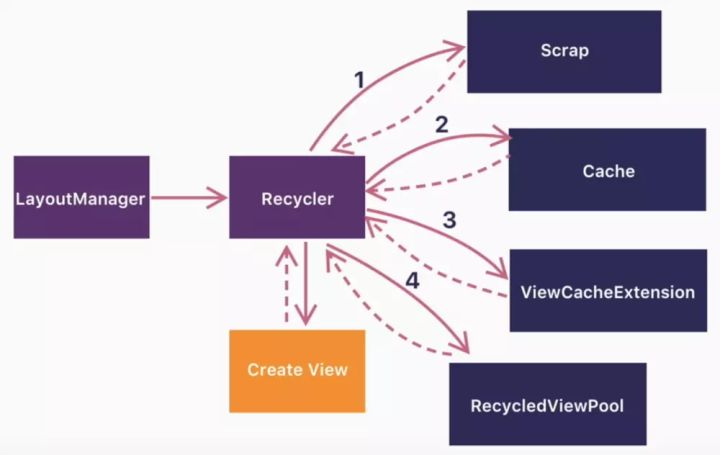
\includegraphics[width=.9\linewidth]{./pic/recyclerviewcache.jpg}

\begin{itemize}
\item Scrap: 在屏幕内可视的Item。
\item Cache: 在屏幕外的Item
\item ViewCacheExtension : 用户自定义的缓存策略
\item RecycledViewPool : 被废弃的itemview,脏数据,需要重新onBindViewHolder.
\item Recycler缓存ViewHolder对象有4个等级,优先级从高到底依次为:
\begin{itemize}
\item 1、ArrayList mAttachedScrap --- 缓存屏幕中可见范围的ViewHolder
\item 2、ArrayList mCachedViews ---- 缓存滑动时即将与RecyclerView分离的ViewHolder,按子View的position或id缓存,默认最多存放2个
\item 3、ViewCacheExtension mViewCacheExtension --- 开发者自行实现的缓存
\item 4、RecycledViewPool mRecyclerPool --- ViewHolder缓存池,本质上是一个SparseArray,其中key是ViewType(int类型),value存放的是 ArrayList< ViewHolder>,默认每个ArrayList中最多存放5个ViewHolder。
\end{itemize}

\item RecyclerView滑动时会触发onTouchEvent\#onMove,回收及复用ViewHolder在这里就会开始。我们知道设置RecyclerView时需要设置LayoutManager,LayoutManager负责RecyclerView的布局,包含对ItemView的获取与复用。以LinearLayoutManager为例,当RecyclerView重新布局时会依次执行下面几个方法:
\begin{itemize}
\item onLayoutChildren():对RecyclerView进行布局的入口方法
\item fill(): 负责对剩余空间不断地填充,调用的方法是layoutChunk()
\item layoutChunk():负责填充View,该View最终是通过在缓存类Recycler中找到合适的View的
\end{itemize}
\item 上述的整个调用链:onLayoutChildren()->fill()->layoutChunk()->next()->getViewForPosition(),getViewForPosition()即是是从RecyclerView的回收机制实现类Recycler中获取合适的View,
\item 下面主要就来从看这个Recycler\#getViewForPosition()的实现。
\end{itemize}
\begin{minted}[frame=lines,fontsize=\scriptsize,linenos=false]{java}
@NonNull 
public View getViewForPosition(int position) { 
    return getViewForPosition(position, false); 
} 
View getViewForPosition(int position, boolean dryRun) { 
    return tryGetViewHolderForPositionByDeadline(position, dryRun, FOREVER_NS).itemView; 
}
\end{minted}
\begin{itemize}
\item 他们都会执行tryGetViewHolderForPositionByDeadline函数,继续跟进去:
\end{itemize}
\begin{minted}[frame=lines,fontsize=\scriptsize,linenos=false]{java}
ViewHolder tryGetViewHolderForPositionByDeadline(int position, boolean dryRun, long deadlineNs) { 
    // ...省略     
    boolean fromScrapOrHiddenOrCache = false; 
    ViewHolder holder = null; 
    // 预布局 属于特殊情况 从mChangedScrap中获取ViewHolder 
    if (mState.isPreLayout()) { 
        holder = getChangedScrapViewForPosition(position); 
        fromScrapOrHiddenOrCache = holder != null; 
    } 
    if (holder == null) { 
        // 1、尝试从mAttachedScrap中获取ViewHolder, 此时获取的是屏幕中可见范围中的ViewHolder 
        // 2、mAttachedScrap缓存中没有的话,继续从mCachedViews尝试获取ViewHolder 
        holder = getScrapOrHiddenOrCachedHolderForPosition(position, dryRun); 
        //  ...省略 
    } 
    if (holder == null) { 
        final int offsetPosition = mAdapterHelper.findPositionOffset(position); 
        //  ...省略 
        final int type = mAdapter.getItemViewType(offsetPosition); 
        // 如果Adapter中声明了Id,尝试从id中获取,这里不属于缓存 
        if (mAdapter.hasStableIds()) 
            holder = getScrapOrCachedViewForId(mAdapter.getItemId(offsetPosition), type, dryRun); 
        if (holder == null && mViewCacheExtension != null) { 
            //  3、从自定义缓存mViewCacheExtension中尝试获取ViewHolder,该缓存需要开发者实现 
            final View view = mViewCacheExtension.getViewForPositionAndType(this, position, type); 
            if (view != null) 
                holder = getChildViewHolder(view); 
        } 
        if (holder == null) { //  fallback to pool 
            // 4、从缓存池mRecyclerPool中尝试获取ViewHolder 
            holder = getRecycledViewPool().getRecycledView(type); 
            if (holder != null) { 
                // 如果获取成功,会重置ViewHolder状态,所以需要重新执行Adapter#onBindViewHolder绑定数据 
                holder.resetInternal(); 
                if (FORCE_INVALIDATE_DISPLAY_LIST) 
                    invalidateDisplayListInt(holder); 
            } 
        } 
        if (holder == null) { 
            // ...省略 
            // 5、若以上缓存中都没有找到对应的ViewHolder,最终会调用Adapter中的onCreateViewHolder创建一个 
            holder = mAdapter.createViewHolder(RecyclerView.this, type); 
        } 
    } 
    boolean bound = false; 
    if (mState.isPreLayout() && holder.isBound()) { 
        holder.mPreLayoutPosition = position; 
    } else if (!holder.isBound() || holder.needsUpdate() || holder.isInvalid()) { 
        final int offsetPosition = mAdapterHelper.findPositionOffset(position); 
        // 6、如果需要绑定数据,会调用Adapter#onBindViewHolder来绑定数据 
        bound = tryBindViewHolderByDeadline(holder, offsetPosition, position, deadlineNs); 
    } 
    // ...省略 
    return holder; 
}
\end{minted}

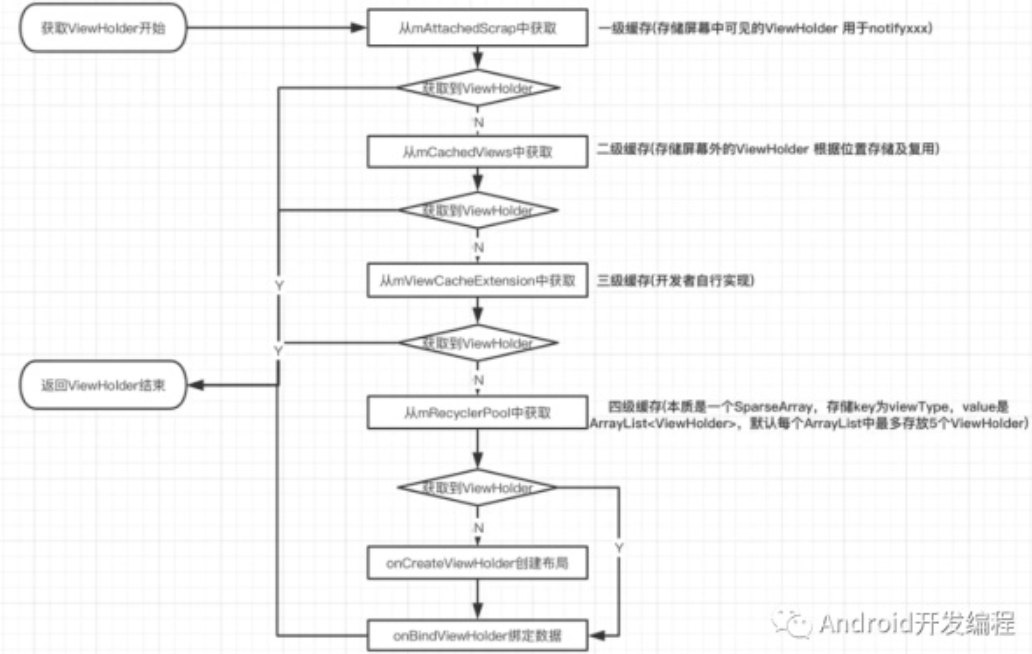
\includegraphics[width=.9\linewidth]{./pic/cache2.png}

\begin{itemize}
\item 通过mAttachedScrap、mCachedViews及mViewCacheExtension获取的ViewHolder不需要重新创建布局及绑定数据;通过缓存池mRecyclerPool获取的ViewHolder不需要重新创建布局,但是需要重新绑定数据;如果上述缓存中都没有获取到目标ViewHolder,那么就会回调Adapter\#onCreateViewHolder()创建布局,以及回调Adapter\#onBindViewHolder()来绑定数据
\item RecyclerView 滑动场景下的回收复用涉及到的结构体两个:
\begin{itemize}
\item mCachedViews 和 RecyclerViewPool
\item mCachedViews 优先级高于 RecyclerViewPool,回收时,最新的 ViewHolder 都是往 mCachedViews 里放,如果它满了,那就移出一个扔到 ViewPool 里好空出位置来缓存最新的 ViewHolder。
\item 复用时,也是先到 mCachedViews 里找 ViewHolder,但需要各种匹配条件,概括一下就是只有原来位置的卡位可以复用存在 mCachedViews 里的 ViewHolder,如果 mCachedViews 里没有,那么才去 ViewPool 里找。
\item 在 ViewPool 里的 ViewHolder 都是跟全新的 ViewHolder 一样,只要 type 一样,有找到,就可以拿出来复用,重新绑定下数据即可。
\end{itemize}
\end{itemize}

\subsection{你可能不知道的RecyclerView性能优化策略}
\label{sec-5-5}
\begin{itemize}
\item 1.不要在onBindViewHolder()中设置监听器,在onCreateViewHolder()中设置监听器.
\item 2.对于使用LinearLayoutManager的情况,做如下设置
\end{itemize}
\begin{minted}[frame=lines,fontsize=\scriptsize,linenos=false]{java}
LinearLayoutManager.setInitialPrefetchitemCount();
\end{minted}
\begin{itemize}
\item 用户滑动到横向滑动的item RecyclerView的时候,由于需要创建更复杂的RecyclerView以及多个子view,可能会导致页面卡顿
\item 由于RenderThread的存在,RecyclerView会进行prefetch
\item LinearLayoutManager.setInitialPrefetchItemCount(int? 横向列表初次显示可见的item个数)
\begin{itemize}
\item 只有LinearLayoutManager有这个API
\item 只有潜逃在内部的RecyclerView才会生效.
\end{itemize}
\item 3.当数据容量固定的时候,设置
\end{itemize}
\begin{minted}[frame=lines,fontsize=\scriptsize,linenos=false]{java}
RecyclerView.setHasFixedSize(true);
// 伪代码
void onContentsChanged() {
    if (mHasFixedSize) 
        layoutChildren();
    else requestLayout();
}
\end{minted}
\begin{itemize}
\item 什么时候用?
\begin{itemize}
\item 如果Adapter的数据变化不会导致RecyclerView的大小变化就可以用
\end{itemize}
\item 4.多个RectclerView共用RecycledViewPool.

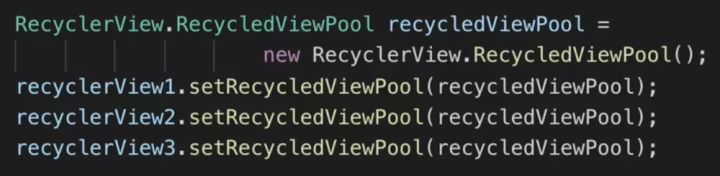
\includegraphics[width=.9\linewidth]{./pic/viewpool.jpg}
\item 5.使用DiffUtil
\end{itemize}
% Emacs 27.1 (Org mode 8.2.7c)
\end{document}